Et magnetometer er et instrument som benyttes for å måle styrken og retningen på det magnetiske feltet som virker på instrumentet. 
Dette kan gjøres på flere måter. De to vanligste typene benytter Hall-effekt eller magnetoresistans for å måle magnetfeltet. \parencite{Skaar2021} 

\subsubsection{Hall-effekt}
Hall-effekten går ut på at ladde partikler i en leder vil trekke mot en av sidene i lederen dersom de blir utsatt for et magnetfelt. 
På grunn av et overskudd av ladde partikler på den ene siden oppstår det en spenningsforskjell på tvers av lederen som 
kan brukes til å måle magnetfelt. Hall-effekten er en utvidelse av Lorentz kraften, som beskriver kraften som påføres en 
ladd partikkel som går gjennom et magnetfelt. Hvis magnetfeltet er orientert vinkelrett på retningen av partikkelens bevegelse, 
vil partikkelen oppleve en kraft som er vinkelrett på både bevegelsesretningen og orienteringen av det magnetiske feltet. \parencite{Keim2015}

\begin{figure}[htp]
\centering
\includegraphics[width=0.5\columnwidth]{figures/hall-sensor}
\caption{Hall-sensor. \parencite{Bosch}}
\label{fig:hall-sensor}
\end{figure}

En Hall-sensor er i sin enkleste form et voltmeter som måler spenningen på tvers av en leder. 
Et magnetometer basert på Hall-effekten benytter typisk to eller flere Hall-sensorer for å kunne 
detektere magnetfelt i et plan eller tredimensjonalt. Dette gjøres ved at sensorene orienteres slik 
at hver sensor måler i hver sin akse, x-y-z. 

\subsubsection{Magnetoresistans}
Magnetoresistans (MR) er en effekt som oppstår når enkelte ledere og halvledere utsettes for et magnetisk felt. 
Alle metaller har en form for MR, men styrken varierer fra metall til metall. 
Effekten går ut på at det oppstår en endring i et metalls elektriske-motstand når et magnetisk felt påvirker metallet. 
Et MR-kompass vil i likhet med Hall-kompass benytte flere sensorer for å nøyaktig måle retningen til jordens magnetiske felt.
MR skiller seg fra Hall-effekt ved at den måler parallelle magnetfelt i motsetning til vinkelrette magnetfelt. 
Dette gjør at en MR-sensor vil oppnå et større deteksjonsfelt. 
I tillegg har en MR-sensor høyere sensitivitet og lavere strømforbruk enn en Hall-sensor. \parencite{ROHM}

\subsubsection{Magnetfelt}

\begin{figure}[htp]
\centering
\includegraphics[width=0.5\columnwidth]{figures/magnetisk-nordpol}
\caption{Posisjonen til den magnetiske Nordpolen de siste 100 årene. \parencite{IncEncyclopediaBritannica}}
\label{fig:magnetisk-nordpol}
\end{figure}

Det er viktig å forstå forskjellen mellom magnetisk nord og faktisk nord ved orientering basert på jordens magnetiske felt. 
Jordens magnetiske felt varierer fra plass til plass og derfor er det avvik mellom faktisk nord og magnetisk nord. 
Den magnetiske Nordpolen er ikke et fast punkt som den faktiske Nordpolen. Den magnetiske Nordpolen flytter på seg over tid, 
og avhenger blant annet av hvordan jordens masse forflytter seg. Dette vil si at magma under de tektoniske platene og 
vann/is vil påvirke hvordan den magnetiske polen forflytter seg . Figur \ref{fig:magnetisk-nordpol} viser hvordan 
den magnetiske Nordpolen har forflyttet seg det siste århundret. 
I tillegg til avvik mellom polene og magnetfeltet er det også lokale variasjoner som gjør at kompass kan vise feil. 
Dette kan komme av lokale ansamlinger av metaller i jordskorpen eller bygninger i urbane miljøer. 
I 2007 utførte NGU en aeromagnetisk undersøkelse over Tromsø for å kartlegge variasjoner i de lokale magnetfeltet. 
Resultatet av denne undersøkelsen vises i figur \ref{fig:magnetisk-nordpol}. Undersøkelsen viser at blant annet områder på Kvaløya og 
Senja har økt magnetfelt i forhold til andre plasser. Derfor er det tenkelig at kompassmisvisningen vil være større i disse områdene. 
\parencite{Kartverket} 

\begin{figure}[htp]
\centering
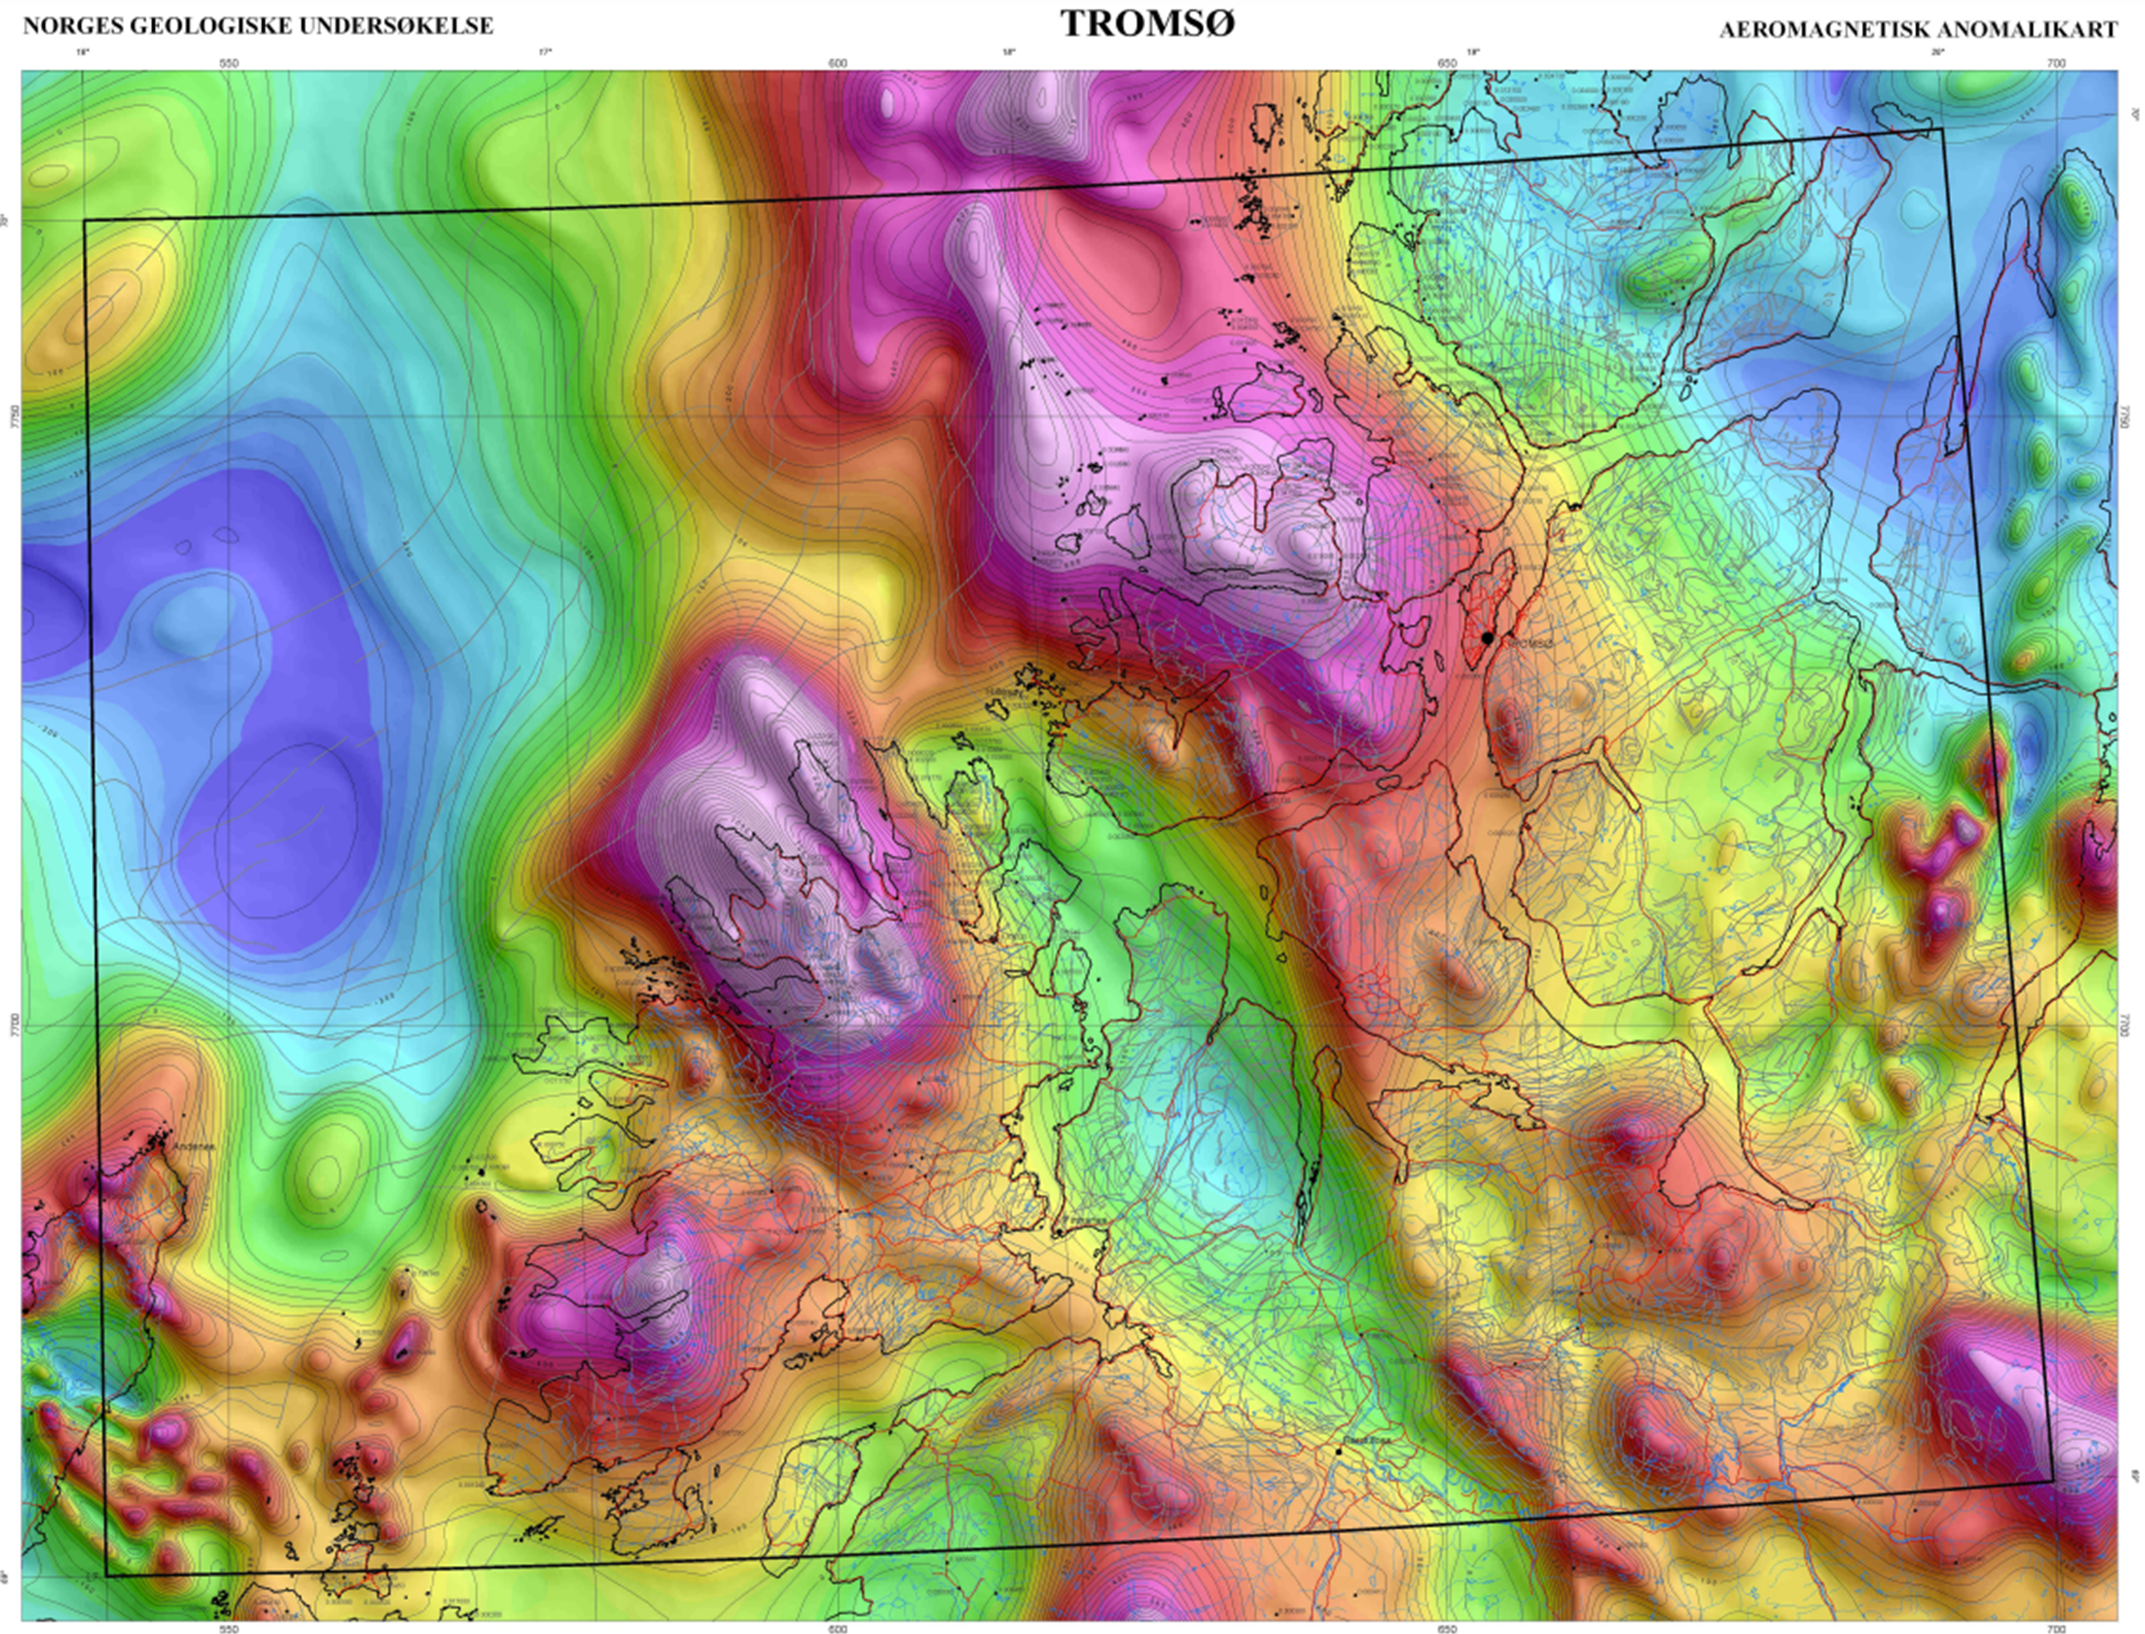
\includegraphics[width=0.5\columnwidth]{figures/aeromagnetisk-kart}
\caption{Aeromagnetisk anomalikart fra undersøkelsen utført av NGU i 2007. \parencite{Gellein2007}}
\label{fig:aeromagnetisk-kart}
\end{figure}